\documentclass[class=article,crop=false]{standalone} \usepackage[margin=1in,headheight=57pt,headsep=0.1in]{geometry}
\usepackage[subpreambles=true]{standalone}
\usepackage{float}
\usepackage[framemethod=TikZ]{mdframed}
\usepackage{fancyhdr}
\usepackage[utf8]{inputenc} % Required for inputting international characters
\usepackage[T1]{fontenc} % Output font encoding for international characters
\usepackage{stix} % Use the STIX fonts
\usepackage{hyperref}
\hbadness=99999

\begin{document}
\subsection{Edit Moves Form}
This is the form that is opened when you click the "Edit Moves" button within the Edit Tile form.
\begin{figure}[H]
	\centering
	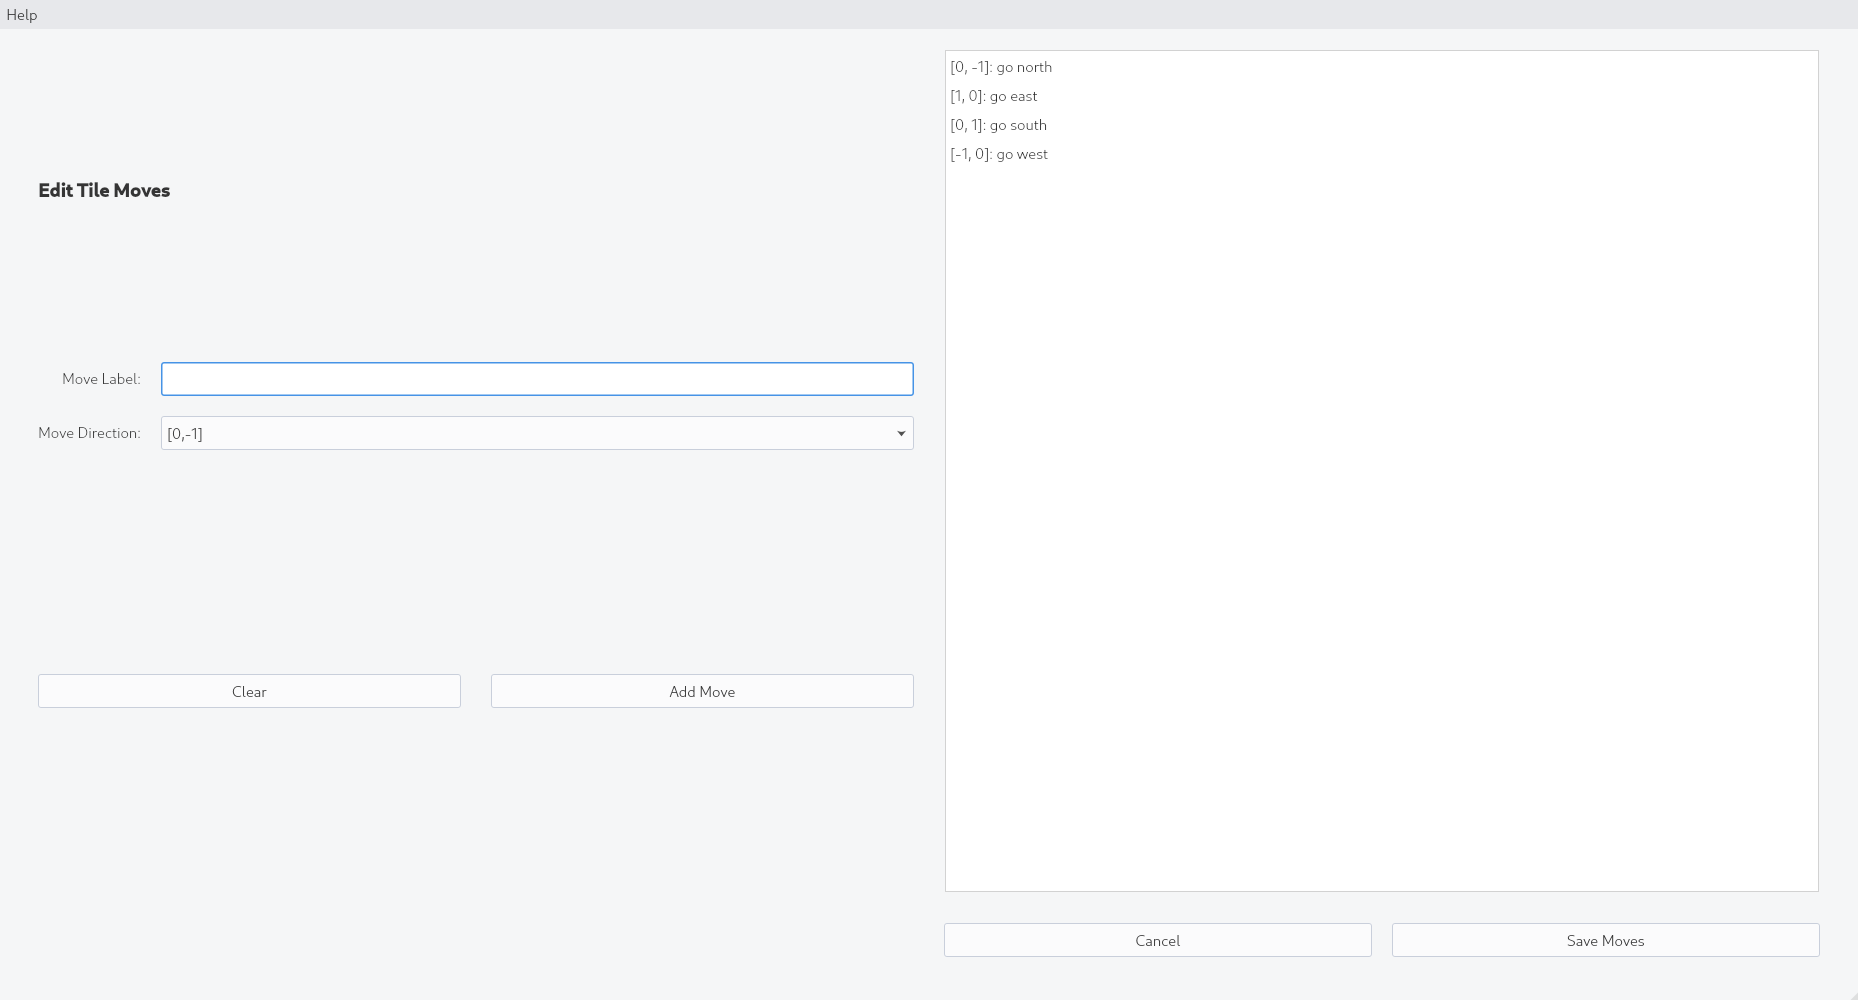
\includegraphics[width=1.0\textwidth]{./editMovesForm.png}
\end{figure}
\begin{itemize}
	\item Move Label: the name of the move as seen by the player. The move is executed after the player enters the move label into the game's text prompt. The label of a move, like the name of a tile, is a unique identifier and reusing a label will result in overwriting the move that previously shared the label.
	\item Move Direction: the "coordinate delta" of the move which as explained in section 2.2, mathematically represents the change in X,Y coordinates which is applied to the player after they execute the move.
	\item "Clear" button: erases the current list of moves for the tile being edited. If this is clicked accidentally, simply cancel the Edit Moves form and reopen it from the Edit Tile form.
	\item "Add Move" button: adds the new individual move (as defined by the label and direction specified in the above input fields) to the tile's overall list of moves.
	\item Cancel: closes the form without saving changes.
	\item Save Moves: closes the form while saving the updated moves to the parent Edit Tile form.
	\item On the right-hand side of the form there is a large read-only list box which displays the list of moves currently assigned to the tile being edited.
\end{itemize}
\end{document}
